\emph{Symmetry breaking} plays a key role in SAT solving by reducing the search space of satisfying assignments for a formula~\cite{biereHandbookSatisfiabilityVolume2009,Crawford},
thus making a wider range of formulas practical to solve.
For example, if one proves that all satisfying assignments to a formula $\phi$ have either (i) $x_1 = 0, x_2 = 1$, or  (ii) $x_1 = 1, x_2 = 0$, and that there is a bijection between satisfying assignments of forms (i) and (ii),
then one can assume, \emph{without loss of generality}, that $x_1 = 0, x_2 = 1$, and thus add unit clauses $\ov{x_1}$ and $x_2$ to the formula $\phi$ while preserving its satisfiability.
There are several techniques that can automatically find symmetry-breaking clauses,
such as structured bounded variable addition~\cite{sbva},
but it is accepted wisdom in the SAT-solving community that problem-specific symmetry breaking is more effective.

In their proof of the Empty Hexagon Number,
Heule and Scheucher showed that for any list of points in general position,
there exists a list of points in \emph{canonical position} with the same triple-orientations.
Canonical position is defined as follows.
\begin{definition}[Canonical Position]
A list of points~$L = (p_1,\ldots, p_{n})$ is said to be in \emph{canonical position} if it satisfies all the following properties:
\begin{itemize}
    \item \textbf{(General Position)} No three points are collinear, i.e., for all $1 \leq i < j < k \leq n$, we have $\sigma(p_i, p_j, p_k) \neq 0$.
    \item \textbf{($x$-order)} The points are sorted with respect to their $x$-coordinates, i.e., $x(p_i) < x(p_j)$ for all $1 \leq i < j \leq n$.
    \item \textbf{(CCW-order)} All orientations $\sigma(p_1, p_i, p_j)$, with $1 < i < j \leq n$, are counterclockwise.
    \item \textbf{(Lex-order)} The list of orientations \( \left(\sigma\left(p_{\lceil \frac{n}{2} \rceil -1}, p_{\lceil \frac{n}{2} \rceil},p_{\lceil \frac{n}{2} \rceil+1}\right), \ldots, \sigma\left(p_2, p_3, p_4\right) \right)\) is not lexicographically smaller than the list \(\left(\sigma\left(p_{\lfloor \frac{n}{2} \rfloor  + 1}, p_{\lfloor \frac{n}{2} \rfloor+2},p_{\lfloor \frac{n}{2} \rfloor+3}\right), \ldots, \sigma\left(p_{n-2}, p_{n-1}, p_{n}\right) \right).\)
    % Given the general position condition, all orientations are in $\{-1, 1\}$, and thus the lexicographic condition is equivalent to stating that there is an index $i$ such that $\forall j < i$, $\textsf{Left}[j] = \textsf{Right}[j]$, and $\textsf{Left}[i] = -1$ but $\textsf{Right}[i] = 1$.
\end{itemize}
\end{definition}

The three ordering properties each break a different symmetry.
First, the $x$-order property breaks symmetry due to how we label the points by ensuring that the points are labeled from left to right.
The $x$-order property also simplifies the encoding of clauses~\labelcref{eq:insideClauses1,eq:insideClauses2,eq:holeDefClauses1,eq:signotopeClauses11,eq:signotopeClauses12},
as they rely on the points being sorted.
Second, the CCW-order property breaks symmetry due to \emph{rotation} by fixing the orientations involving the leftmost point~$p_1$.

\begin{figure}
    \centering
    \begin{subfigure}{0.3\linewidth}
        \centering
        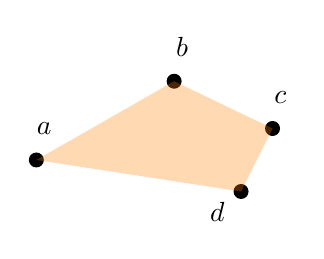
\begin{tikzpicture}
            \node[draw, circle, black, fill=black, inner sep=0pt, minimum size=5pt, label={[xshift=0.1cm, yshift=0.1cm]$a$}] (a) at (0,0) {};
            \node[draw, circle, black, fill=black, inner sep=0pt, minimum size=5pt, label={[xshift=0.1cm, yshift=0.1cm]$b$}] (b) at (1.75,1) {};
            \node[draw, circle, black, fill=black, inner sep=0pt, minimum size=5pt, label={[xshift=0.1cm, yshift=0.1cm]$c$}] (c) at (3,0.4) {};
            \node[draw, circle, black, fill=black, inner sep=0pt, minimum size=5pt, label={[xshift=-0.3cm, yshift=-0.6cm]$d$}] (d) at (2.6,-0.4) {};
            \coordinate (a) at (0,0);
            \coordinate (b) at (1.75,1);
            \coordinate (c) at (3,0.4);
            \coordinate (d) at (2.6,-0.4);
            \fill[orange, opacity=0.3] (a) -- (b) -- (c) -- (d) -- (a) -- cycle;
        \end{tikzpicture}
        \caption{The signature induced by $\sigma$ is $\texttt{-\,-\,-\,-}$.}
    \end{subfigure}
    \begin{subfigure}{0.3\linewidth}
        \centering
        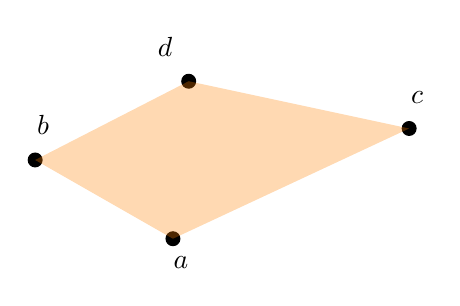
\begin{tikzpicture}
            \node[draw, circle, black, fill=black, inner sep=0pt, minimum size=5pt, label={[xshift=0.1cm, yshift=-0.6cm]$a$}] (a) at (0,0) {};
            \node[draw, circle, black, fill=black, inner sep=0pt, minimum size=5pt, label={[xshift=0.1cm, yshift=0.1cm]$b$}] (b) at (-1.75,1) {};
            \node[draw, circle, black, fill=black, inner sep=0pt, minimum size=5pt, label={[xshift=0.1cm, yshift=0.1cm]$c$}] (c) at (3,1.4) {};
            \node[draw, circle, black, fill=black, inner sep=0pt, minimum size=5pt, label={[xshift=-0.3cm, yshift=0.1cm]$d$}] (d) at (0.2,2) {};
            \coordinate (a) at (0,0);
            \coordinate (b) at (-1.75,1);
            \coordinate (c) at (3,1.4);
            \coordinate (d) at (0.2,2);
            \fill[orange, opacity=0.3] (b) -- (d) -- (c) -- (a) -- (b) -- cycle;
        \end{tikzpicture}
        \caption{The signature induced by $\sigma$ is $\texttt{-\,-\,+\,-}$.}
    \end{subfigure}
    \begin{subfigure}{0.3\linewidth}
        \centering
        
\begin{tikzpicture}
            \node[draw, circle, black, fill=black, inner sep=0pt, minimum size=5pt] (p) at (0,0) {};
        \end{tikzpicture}
    \end{subfigure}
  \caption{Illustration of the notion of $\sigma$-equivalence.}\label{fig:sigma-equiv}
  \end{figure}


Third, the lex-order property breaks symmetry due to \emph{reflection}.
Reflecting a set of points~$S$ over a line (e.g., with the map $(x, y) \mapsto (-x, y)$)
preserves the presence of $k$-holes and convex $k$-gons.
This operation does not quite preserve orientations, but rather flips them
(clockwise orientations become counterclockwise and vice versa).
Our definition of $\sigma$-equivalence includes a \emph{parity} flag for this purpose:
\lstinline|parity := false| corresponds to the case that orientations are the same,
and \lstinline|parity := true| corresponds to the case that all orientations have been flipped.
See the point sets in \Cref{fig:sigma-equiv} for an example.

The lex-order property, then, picks between a set of points and its reflection over \(x=0\).
The vector of consecutive orientations from the middle to the left
is assumed to be at least as big as the vector of consecutive orientations from the middle to the right.
This constraint is not geometrically meaningful,
but is easy to implement in the SAT encoding.

We prove that there always exists a $\sigma$-equivalent point set in canonical position.

%     While the first 3 conditions are now arguably standard in computational results regarding Erd\H{o}s-Szekeres type problems~\cite{scheucherTwoDisjoint5holes2020}, the last condition is a novelty introduced by Heule and Scheucher.
%     Interestingly, in the process of verifying the correctness of this symmetry-breaking assumption, we found a small error in the proof presented in~\cite{scheucherTwoDisjoint5holes2020} for the first $3$ conditions.
% The concrete theorem we prove is the following:
\begin{figure}[t]
\begin{subfigure}{0.31\textwidth}
\centering
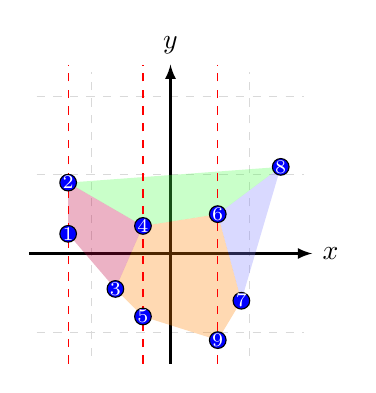
\begin{tikzpicture}
        \draw[help lines, color=gray!30, dashed] (-1.7,-1.3) grid (1.7,2.3);
    \draw[-latex, thick] (-1.8,0)--(1.8,0) node[right]{$x$};
    \draw[-latex, thick] (0,-1.4)--(0,2.4) node[above]{$y$};

    \coordinate (c1) at (-1.3, 0.25);
    \coordinate (c2) at (-1.3, 0.9);
    \coordinate (c3) at (-0.7, -0.45);
    \coordinate (c4) at (-0.35, 0.35);
    \coordinate (c5) at (-0.35, -0.8);
    \coordinate (c6) at (0.6, 0.5);
    \coordinate (c7) at (0.9, -0.6);
    \coordinate (c8) at (1.4, 1.1);
    \coordinate (c9) at (0.6, -1.1);
    
    \fill[orange, opacity=0.3] (c3) -- (c4) -- (c6) -- (c7) -- (c9) -- (c5) -- (c3) -- cycle;
    \fill[purple, opacity=0.3] (c2) -- (c4) -- (c3) -- (c1) -- (c2) -- cycle;
    \fill[blue!50!white, opacity=0.3] (c6) -- (c7) -- (c8) -- (c6) -- cycle;
    \fill[green!70!white, opacity=0.3] (c2) -- (c4) -- (c6) -- (c8) -- (c2) -- cycle;
 
    \draw[-, dashed, red] (-1.3, -1.4) -- (-1.3, 2.4);
    \draw[-, dashed, red] (-0.35, -1.4) -- (-0.35, 2.4);
    \draw[-, dashed, red] (0.6, -1.4) -- (0.6, 2.4);
    \node[draw, circle, fill=blue, text=white, inner sep=0pt, minimum size=5pt] (p1) at (-1.3, 0.25) {\scriptsize $1$};
    \node[draw, circle, fill=blue, text=white, inner sep=0pt, minimum size=5pt] (p2) at (-1.3, 0.9) {\scriptsize $2$};
    \node[draw, circle, fill=blue, text=white, inner sep=0pt, minimum size=5pt] (p3) at (-0.7, -0.45) {\scriptsize $3$};
    \node[draw, circle, fill=blue, text=white, inner sep=0pt, minimum size=5pt] (p4) at (-0.35, 0.35) {\scriptsize $4$};
    \node[draw, circle, fill=blue, text=white, inner sep=0pt, minimum size=5pt] (p5) at (-0.35, -0.8) {\scriptsize $5$};
    \node[draw, circle, fill=blue, text=white, inner sep=0pt, minimum size=5pt] (p6) at (0.6, 0.5) {\scriptsize $6$};
    \node[draw, circle, fill=blue, text=white, inner sep=0pt, minimum size=5pt] (p7) at (0.9, -0.6) {\scriptsize $7$};
    \node[draw, circle, fill=blue, text=white, inner sep=0pt, minimum size=5pt] (p8) at (1.4, 1.1) {\scriptsize $8$};
    \node[draw, circle, fill=blue, text=white, inner sep=0pt, minimum size=5pt] (p9) at (0.6, -1.1) {\scriptsize $9$};
\end{tikzpicture}
\caption{The original list of points.\\\phantom{x}\\\phantom{x}}\label{fig:symmetry-breaking-1}
\end{subfigure}
\hfil
\begin{subfigure}{0.31\textwidth}
    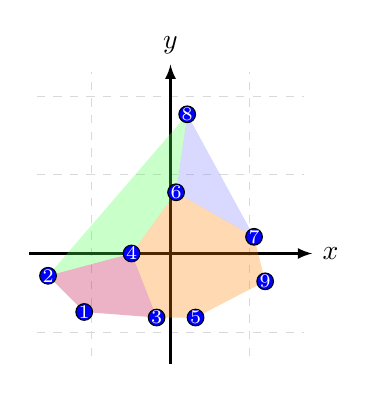
\begin{tikzpicture}
        \draw[help lines, color=gray!30, dashed] (-1.7,-1.3) grid (1.7,2.3);
    \draw[-latex, thick] (-1.8,0)--(1.8,0) node[right]{$x$};
    \draw[-latex, thick] (0,-1.4)--(0,2.4) node[above]{$y$};
    

    \coordinate (c1) at (-1.09601563215555, -0.7424619411597272);
\coordinate (c2) at (-1.5556349648261614, -0.28284245828783905);
\coordinate (c3) at (-0.17677682816699475, -0.8131727694796578);
\coordinate (c4) at (-0.49497474683057663, 8.087761060870946e-08);
\coordinate (c5) at (0.3181979186635819, -0.8131728503572684);
\coordinate (c6) at (0.07071080521204193, 0.7778174477512475);
\coordinate (c7) at (1.0606602064416402, 0.21213186104679588);
\coordinate (c8) at (0.21213232320457065, 1.767766918304512);
\coordinate (c9) at (1.202081470247393, -0.3535535870103234);

\fill[orange, opacity=0.3] (c3) -- (c4) -- (c6) -- (c7) -- (c9) -- (c5) -- (c3) -- cycle;
\fill[purple, opacity=0.3] (c2) -- (c4) -- (c3) -- (c1) -- (c2) -- cycle;
\fill[blue!50!white, opacity=0.3] (c6) -- (c7) -- (c8) -- (c6) -- cycle;
\fill[green!70!white, opacity=0.3] (c2) -- (c4) -- (c6) -- (c8) -- (c2) -- cycle;

        \node[draw, circle, fill=blue, text=white, inner sep=0pt, minimum size=5pt] (p1) at (-1.09601563215555, -0.7424619411597272) {\scriptsize $1$};
        \node[draw, circle, fill=blue, text=white, inner sep=0pt, minimum size=5pt] (p2) at (-1.5556349648261614, -0.28284245828783905) {\scriptsize $2$};
        \node[draw, circle, fill=blue, text=white, inner sep=0pt, minimum size=5pt] (p3) at (-0.17677682816699475, -0.8131727694796578) {\scriptsize $3$};
        \node[draw, circle, fill=blue, text=white, inner sep=0pt, minimum size=5pt] (p4) at (-0.49497474683057663, 8.087761060870946e-08) {\scriptsize $4$};
        \node[draw, circle, fill=blue, text=white, inner sep=0pt, minimum size=5pt] (p5) at (0.3181979186635819, -0.8131728503572684) {\scriptsize $5$};
        \node[draw, circle, fill=blue, text=white, inner sep=0pt, minimum size=5pt] (p6) at (0.07071080521204193, 0.7778174477512475) {\scriptsize $6$};
        \node[draw, circle, fill=blue, text=white, inner sep=0pt, minimum size=5pt] (p7) at (1.0606602064416402, 0.21213186104679588) {\scriptsize $7$};
        \node[draw, circle, fill=blue, text=white, inner sep=0pt, minimum size=5pt] (p8) at (0.21213232320457065, 1.767766918304512) {\scriptsize $8$};
        \node[draw, circle, fill=blue, text=white, inner sep=0pt, minimum size=5pt] (p9) at (1.202081470247393, -0.3535535870103234) {\scriptsize $9$};
    \end{tikzpicture}

\caption{All $x$-coordinates are different after rotating by $45^\circ$. We show such an angle always exists.}\label{fig:symmetry-breaking-2}
\end{subfigure}
\hfil
%
%\vspace{0.5cm}
%
\begin{subfigure}{0.31\textwidth}
    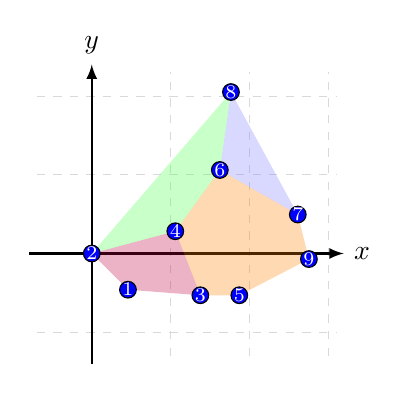
\begin{tikzpicture}
            \draw[help lines, color=gray!30, dashed] (-0.7,-1.3) grid (3.1,2.3);
    \draw[-latex, thick] (-0.8,0)--(3.2,0) node[right]{$x$};
    \draw[-latex, thick] (0,-1.4)--(0,2.4) node[above]{$y$};
    
    \coordinate (c1) at (0.4596193326706113, -0.45961948287188814);
\coordinate (c2) at (0.0, 0.0);
\coordinate (c3) at (1.3788581366591666, -0.5303303111918187);
\coordinate (c4) at (1.0606602179955846, 0.28284253916544966);
\coordinate (c5) at (1.8738328834897433, -0.5303303920694293);
\coordinate (c6) at (1.6263457700382034, 1.0606599060390867);
\coordinate (c7) at (2.6162951712678018, 0.4949743193346349);
\coordinate (c8) at (1.767767288030732, 2.0506093765923508);
\coordinate (c9) at (2.7577164350735544, -0.07071112872248436);

\fill[orange, opacity=0.3] (c3) -- (c4) -- (c6) -- (c7) -- (c9) -- (c5) -- (c3) -- cycle;
\fill[purple, opacity=0.3] (c2) -- (c4) -- (c3) -- (c1) -- (c2) -- cycle;
\fill[blue!50!white, opacity=0.3] (c6) -- (c7) -- (c8) -- (c6) -- cycle;
\fill[green!70!white, opacity=0.3] (c2) -- (c4) -- (c6) -- (c8) -- (c2) -- cycle;
%        \draw[help lines, color=gray!30, dashed] (-1,-0.9) grid (2.9,2.4);
%        \draw[-latex, thick] (-1,0)--(4,0) node[right]{$x$};
%        \draw[-latex, thick] (0,-1)--(0,2.5) node[above]{$y$};
    
        \node[draw, circle, fill=blue, text=white, inner sep=0pt, minimum size=5pt] (p1) at (0.4596193326706113, -0.45961948287188814) {\scriptsize $1$};
        \node[draw, circle, fill=blue, text=white, inner sep=0pt, minimum size=5pt] (p2) at (0.0, 0.0) {\scriptsize $2$};
        \node[draw, circle, fill=blue, text=white, inner sep=0pt, minimum size=5pt] (p3) at (1.3788581366591666, -0.5303303111918187) {\scriptsize $3$};
        \node[draw, circle, fill=blue, text=white, inner sep=0pt, minimum size=5pt] (p4) at (1.0606602179955846, 0.28284253916544966) {\scriptsize $4$};
        \node[draw, circle, fill=blue, text=white, inner sep=0pt, minimum size=5pt] (p5) at (1.8738328834897433, -0.5303303920694293) {\scriptsize $5$};
        \node[draw, circle, fill=blue, text=white, inner sep=0pt, minimum size=5pt] (p6) at (1.6263457700382034, 1.0606599060390867) {\scriptsize $6$};
        \node[draw, circle, fill=blue, text=white, inner sep=0pt, minimum size=5pt] (p7) at (2.6162951712678018, 0.4949743193346349) {\scriptsize $7$};
        \node[draw, circle, fill=blue, text=white, inner sep=0pt, minimum size=5pt] (p8) at (1.767767288030732, 2.0506093765923508) {\scriptsize $8$};
        \node[draw, circle, fill=blue, text=white, inner sep=0pt, minimum size=5pt] (p9) at (2.7577164350735544, -0.07071112872248436) {\scriptsize $9$};
    \end{tikzpicture}

\caption{After translating, the leftmost point is at $(0,0)$.\\\phantom{x}}\label{fig:symmetry-breaking-3}
\end{subfigure}

\begin{subfigure}{0.31\textwidth}
    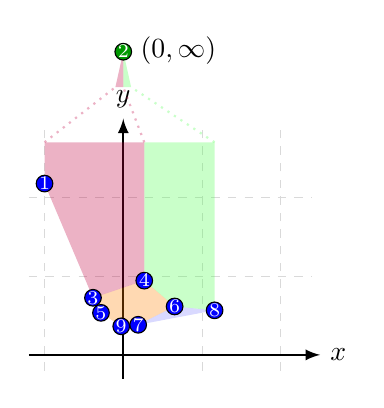
\begin{tikzpicture}
        \draw[help lines, color=gray!30, dashed] (-1.2,-0.2) grid (2.4,2.9);
        \draw[-latex, thick] (-1.2,0)--(2.5,0) node[right]{$x$};
        \draw[-latex, thick] (0,-0.3)--(0,3) node[above]{$y$};
    
        \coordinate (c1) at (-1.00000032679495, 2.1757135283877527);
\coordinate (c2) at (0, 3.85);
\coordinate (c2-1) at (-1.00000032679495, 2.7);
\coordinate (c2-4) at (0.2666664916498519, 2.7);
\coordinate (c2-8) at (1.1599996167350177, 2.7);
\coordinate (t-c2-1) at (-0.1, 3.4);
\coordinate (t-c2-4) at (0, 3.4);
\coordinate (t-c2-8) at (0.1, 3.4);
\coordinate (c3) at (-0.3846155721840648, 0.7252377698715973);
\coordinate (c4) at (0.2666664916498519, 0.9428090005013866);
\coordinate (c5) at (-0.2830190444100679, 0.5336655199142649);
\coordinate (c6) at (0.6521736801480853, 0.6148753963780468);
\coordinate (c7) at (0.1891890199433349, 0.3822198699068886);
\coordinate (c8) at (1.1599996167350177, 0.5656853177286622);
\coordinate (c9) at (-0.025641189145902285, 0.3626188636662086);

\fill[orange, opacity=0.3] (c3) -- (c4) -- (c6) -- (c7) -- (c9) -- (c5) -- (c3) -- cycle;
\fill[blue!50!white, opacity=0.3] (c6) -- (c7) -- (c8) -- (c6) -- cycle;
\fill[purple, opacity=0.3] (c2-4) -- (c4) -- (c3) -- (c1) -- (c2-1) -- cycle;
\fill[purple, opacity=0.3] (t-c2-1) -- (c2) -- (t-c2-4) -- (t-c2-1) -- cycle;
\fill[green!70!white, opacity=0.3] (t-c2-4) -- (c2) -- (t-c2-8) -- (t-c2-4) -- cycle;
\fill[green!70!white, opacity=0.3] (c2-4) -- (c4) -- (c6) -- (c8) -- (c2-8) -- cycle;

\draw[thick, dotted,purple, opacity=0.3] (c2-1) -- (t-c2-1);
\draw[thick, dotted, purple, opacity=0.3] (c2-4) -- (t-c2-4);
\draw[thick, dotted, green!70!white, opacity=0.3] (c2-8) -- (t-c2-8);


        \node[draw, circle, fill=blue, text=white, inner sep=0pt, minimum size=5pt] (p1) at (-1.00000032679495, 2.1757135283877527) {\scriptsize $1$};
        \node[draw, circle, fill=green!60!black, text=white, inner sep=0pt, minimum size=5pt, label={[xshift=0.7cm, yshift=-0.4cm]$(0, \infty)$}] (p2) at (0, 3.85) {\scriptsize $2$};
        \node[draw, circle, fill=blue, text=white, inner sep=0pt, minimum size=5pt] (p3) at (-0.3846155721840648, 0.7252377698715973) {\scriptsize $3$};
        \node[draw, circle, fill=blue, text=white, inner sep=0pt, minimum size=5pt] (p4) at (0.2666664916498519, 0.9428090005013866) {\scriptsize $4$};
        \node[draw, circle, fill=blue, text=white, inner sep=0pt, minimum size=5pt] (p5) at (-0.2830190444100679, 0.5336655199142649) {\scriptsize $5$};
        \node[draw, circle, fill=blue, text=white, inner sep=0pt, minimum size=5pt] (p6) at (0.6521736801480853, 0.6148753963780468) {\scriptsize $6$};
        \node[draw, circle, fill=blue, text=white, inner sep=0pt, minimum size=5pt] (p7) at (0.1891890199433349, 0.3822198699068886) {\scriptsize $7$};
        \node[draw, circle, fill=blue, text=white, inner sep=0pt, minimum size=5pt] (p8) at (1.1599996167350177, 0.5656853177286622) {\scriptsize $8$};
        \node[draw, circle, fill=blue, text=white, inner sep=0pt, minimum size=5pt] (p9) at (-0.025641189145902285, 0.3626188636662086) {\scriptsize $9$};
       
    \end{tikzpicture}

\caption{Result after applying the map $(x, y) \mapsto (y/x, 1/x)$.}\label{fig:symmetry-breaking-4}
\end{subfigure}
\hfil
%
%\vspace{0.5cm}
%
\begin{subfigure}{0.31\textwidth}
    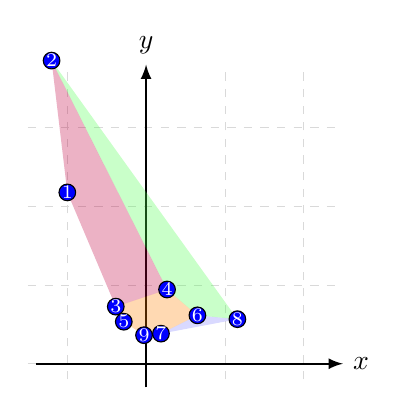
\begin{tikzpicture}
        \draw[help lines, color=gray!30, dashed] (-1.5,-0.2) grid (2.4,3.7);
        \draw[-latex, thick] (-1.4,0)--(2.5,0) node[right]{$x$};
        \draw[-latex, thick] (0,-0.3)--(0,3.8) node[above]{$y$};
    
        \coordinate (c1) at (-1.00000032679495, 2.1757135283877527);
        \coordinate (c2) at (-1.2, 3.85);
        \coordinate (c3) at (-0.3846155721840648, 0.7252377698715973);
        \coordinate (c4) at (0.2666664916498519, 0.9428090005013866);
        \coordinate (c5) at (-0.2830190444100679, 0.5336655199142649);
        \coordinate (c6) at (0.6521736801480853, 0.6148753963780468);
        \coordinate (c7) at (0.1891890199433349, 0.3822198699068886);
        \coordinate (c8) at (1.1599996167350177, 0.5656853177286622);
        \coordinate (c9) at (-0.025641189145902285, 0.3626188636662086);
   
        \fill[orange, opacity=0.3] (c3) -- (c4) -- (c6) -- (c7) -- (c9) -- (c5) -- (c3) -- cycle;
        \fill[blue!50!white, opacity=0.3] (c6) -- (c7) -- (c8) -- (c6) -- cycle;
        \fill[purple, opacity=0.3] (c2) -- (c4) -- (c3) -- (c1) -- (c2) -- cycle;
        \fill[green!70!white, opacity=0.3] (c2) -- (c4) -- (c6) -- (c8) -- (c2) -- cycle;

        \node[draw, circle, fill=blue, text=white, inner sep=0pt, minimum size=5pt] (p1) at (-1.00000032679495, 2.1757135283877527) {\scriptsize $1$};
        \node[draw, circle, fill=blue, text=white, inner sep=0pt, minimum size=5pt] (p2) at (-1.2, 3.85) {\scriptsize $2$};
        \node[draw, circle, fill=blue, text=white, inner sep=0pt, minimum size=5pt] (p3) at (-0.3846155721840648, 0.7252377698715973) {\scriptsize $3$};
        \node[draw, circle, fill=blue, text=white, inner sep=0pt, minimum size=5pt] (p4) at (0.2666664916498519, 0.9428090005013866) {\scriptsize $4$};
        \node[draw, circle, fill=blue, text=white, inner sep=0pt, minimum size=5pt] (p5) at (-0.2830190444100679, 0.5336655199142649) {\scriptsize $5$};
        \node[draw, circle, fill=blue, text=white, inner sep=0pt, minimum size=5pt] (p6) at (0.6521736801480853, 0.6148753963780468) {\scriptsize $6$};
        \node[draw, circle, fill=blue, text=white, inner sep=0pt, minimum size=5pt] (p7) at (0.1891890199433349, 0.3822198699068886) {\scriptsize $7$};
        \node[draw, circle, fill=blue, text=white, inner sep=0pt, minimum size=5pt] (p8) at (1.1599996167350177, 0.5656853177286622) {\scriptsize $8$};
        \node[draw, circle, fill=blue, text=white, inner sep=0pt, minimum size=5pt] (p9) at (-0.025641189145902285, 0.3626188636662086) {\scriptsize $9$};
       
       

    \end{tikzpicture}

\caption{Point $2$ is brought back into the real plane.}\label{fig:symmetry-breaking-5}
\end{subfigure}
\hfil
\begin{subfigure}{0.31\textwidth}
    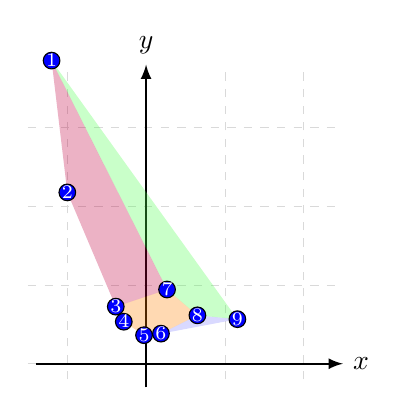
\begin{tikzpicture}
        \draw[help lines, color=gray!30, dashed] (-1.5,-0.2) grid (2.4,3.7);
        \draw[-latex, thick] (-1.4,0)--(2.5,0) node[right]{$x$};
        \draw[-latex, thick] (0,-0.3)--(0,3.8) node[above]{$y$};
    
        \coordinate (c1) at (-1.00000032679495, 2.1757135283877527);
        \coordinate (c2) at (-1.2, 3.85);
        \coordinate (c3) at (-0.3846155721840648, 0.7252377698715973);
        \coordinate (c4) at (0.2666664916498519, 0.9428090005013866);
        \coordinate (c5) at (-0.2830190444100679, 0.5336655199142649);
        \coordinate (c6) at (0.6521736801480853, 0.6148753963780468);
        \coordinate (c7) at (0.1891890199433349, 0.3822198699068886);
        \coordinate (c8) at (1.1599996167350177, 0.5656853177286622);
        \coordinate (c9) at (-0.025641189145902285, 0.3626188636662086);
        
        \fill[orange, opacity=0.3] (c3) -- (c4) -- (c6) -- (c7) -- (c9) -- (c5) -- (c3) -- cycle;
        \fill[blue!50!white, opacity=0.3] (c6) -- (c7) -- (c8) -- (c6) -- cycle;
        \fill[purple, opacity=0.3] (c2) -- (c4) -- (c3) -- (c1) -- (c2) -- cycle;
    \fill[green!70!white, opacity=0.3] (c2) -- (c4) -- (c6) -- (c8) -- (c2) -- cycle;

        \node[draw, circle, fill=blue, text=white, inner sep=0pt, minimum size=5pt] (p1) at (-1.2, 3.85) {\scriptsize $1$};
        \node[draw, circle, fill=blue, text=white, inner sep=0pt, minimum size=5pt] (p2) at (-1.00000032679495, 2.1757135283877527) {\scriptsize $2$};
        \node[draw, circle, fill=blue, text=white, inner sep=0pt, minimum size=5pt] (p3) at (-0.3846155721840648, 0.7252377698715973) {\scriptsize $3$};
        \node[draw, circle, fill=blue, text=white, inner sep=0pt, minimum size=5pt] (p4) at (-0.2830190444100679, 0.5336655199142649) {\scriptsize $4$};
        \node[draw, circle, fill=blue, text=white, inner sep=0pt, minimum size=5pt] (p5) at (-0.025641189145902285, 0.3626188636662086) {\scriptsize $5$};
        \node[draw, circle, fill=blue, text=white, inner sep=0pt, minimum size=5pt] (p6) at (0.1891890199433349, 0.3822198699068886) {\scriptsize $6$};
        \node[draw, circle, fill=blue, text=white, inner sep=0pt, minimum size=5pt] (p7) at (0.2666664916498519, 0.9428090005013866) {\scriptsize $7$};
        \node[draw, circle, fill=blue, text=white, inner sep=0pt, minimum size=5pt] (p8) at (0.6521736801480853, 0.6148753963780468) {\scriptsize $8$};
        \node[draw, circle, fill=blue, text=white, inner sep=0pt, minimum size=5pt] (p9) at (1.1599996167350177, 0.5656853177286622) {\scriptsize $9$};
       
    \end{tikzpicture}

\caption{Points are relabeled from left to right.}\label{fig:symmetry-breaking-6}
\end{subfigure}



\caption{Illustration of the proof of the symmetry breaking theorem. Note that the highlighted holes are preserved as $\sigma$-equivalence is preserved. For simplicity we have ommited the illustration of the \emph{Lex-order} property. }\label{fig:symmetry-breaking}
\end{figure}
\begin{lstlisting}
theorem symmetry_breaking : ListInGenPos l →
  ∃ w : CanonicalPoints, Nonempty (l.toFinset ≃σ w.points.toFinset)
\end{lstlisting}


\begin{proof}[Proof Sketch]
The proof proceeds in 6 steps, illustrated in~\Cref{fig:symmetry-breaking}.
In each of the steps, we construct a new list of points that is $\sigma$-equivalent to the previous one,
with the last one being in canonical position.\footnote{
Even though we defined $\sigma$-equivalence for sets of points,
our formalization goes back and forth between sets and lists.
Given that symmetry breaking distinguishes between the order of the points
e.g., $x$-order, this proof proceeds over lists.
All permutations of a list are immediately $\sigma$-equivalent.}
The main justification for each step is that,
given that the function $\sigma$ is defined as a sign of the determinant,
applying transformations that preserve (or, when \lstinline|parity := true|, uniformly reverse)
the sign of the determinant will preserve (or uniformly reverse) the values of $\sigma$.

For example, given the identity $\det(AB) = \det(A)\det(B)$,
if we apply a transformation to the points that corresponds to multiplying by a matrix $B$ such that $\det(B) > 0$,
then $\sign(\det(A)) = \sign(\det(AB))$, and thus orientations will be preserved.
\textbf{Step 1}: we transform the list of points so that no two points share the same $x$-coordinate.
This can be done by applying a rotation to the list of points, which corresponds to multiplying by a rotation matrix.
Rotations always have determinant $1$.
\textbf{Step 2}: we translate all points by a constant vector $t$, which corresponds to multiplying by a translation matrix,
to bring the leftmost point~$p_1$ to position $(0, 0)$.
As a result, every other point has a positive $x$-coordinate.

Let $L_2$ be the list of points excluding $p_1$ after Step 2.
\textbf{Step 3}: we apply the projective transformation $f: (x, y) \mapsto (y/x, 1/x)$ to every point in $L_2$,
showing that this preserves orientations within $L_2$.
To see that this mapping is a $\sigma$-equivalence consider that
\[
\begin{multlined}
 \sign \det \begin{pmatrix} p_x & q_x & r_x \\ p_y & q_y & r_y \\ 1 & 1 & 1 \end{pmatrix} =  \sign \det \left( \begin{pmatrix} 0 & 0 & 1 \\ 1 & 0 & 0\\ 0 & 1 & 0 \end{pmatrix}  \begin{pmatrix} \nicefrac{p_y}{p_x} & \nicefrac{q_y}{q_x} & \nicefrac{r_y}{r_x} \\ \nicefrac{1}{p_x} & \nicefrac{1}{q_x} & \nicefrac{1}{r_x} \\ 1 & 1 & 1 \end{pmatrix}  \begin{pmatrix} p_x & 0 & 0 \\ 0 & q_x & 0\\ 0 & 0 & r_x \end{pmatrix} \right)\\
                        = \sign \left(1 \cdot \det  \begin{pmatrix} \nicefrac{p_y}{p_x} & \nicefrac{q_y}{q_x} & \nicefrac{r_y}{r_x} \\ \nicefrac{1}{p_x} & \nicefrac{1}{q_x} & \nicefrac{1}{r_x} \\ 1 & 1 & 1 \end{pmatrix} \cdot  p_x q_x r_x  \right) = \sign \det \begin{pmatrix} p_y/p_x & q_y/q_x & r_y/r_x \\ 1/p_x & 1/q_x & 1/r_x \\ 1 & 1 & 1 \end{pmatrix}.
                        %  \tag{As $p_x q_x r_x > 0$ by step 2}
\end{multlined}
\]
To preserve orientations with respect to the leftmost point $(0, 0)$, we set $f( (0, 0)) = (0, \infty)$,
a special point that is treated separately as follows.
As the function $\sigma$ takes points in $\mathbb{R}^2$ as arguments,
we need to define an extension
\(
  \sigma_{(0, \infty)}(q, r) = \begin{cases}
    1 & \text{if } q_x < r_x \\
    -1 & \text{otherwise}.  
  \end{cases},
\)
We then show that $\sigma((0, 0), q, r) = \sigma_{(0, \infty)}(f(q), f(r))$ for all points $q, r \in L_2$. 

\textbf{Step 4}: we sort the list~$L_2$ by $x$-coordinate in increasing order,
thus obtaining a list~$L_3$.
This can be done while preserving $\sigma$-equivalence because sorting corresponds to a permutation,
and all permutations of a list are $\sigma$-equivalent by definition.
\textbf{Step 5}: we check whether the \textsf{Lex order} condition above is satisfied in $L_3$,
and if it is not, we reflect the pointset,
which preserves $\sigma$-equivalence with \lstinline|parity := true|.
Note that in such a case we need to relabel the points from left to right again.

\textbf{Step 6}: we bring point $(0, \infty)$ back into the range
by first finding a constant $c$ such that all points in $L_3$ are to the right of the line $y=c$,
and then finding a large enough value $M$ such that $(c, M)$ has the same orientation
with respect to the other points as $(0, \infty)$ did,
meaning that 
\(\sigma((c, M), q, r) = \sigma_{(0, \infty)}(q, r)\) for every $q, r \in L_3$.

Finally, we note that the list of points obtained in step 6
satisfies the \text{CCW-order} property by the following reasoning:
if $1 < i < j \leq n$ are indices, then 
\begin{align*}
  \sigma(p_1, p_i, p_j) = 1 &\iff \sigma((c, M), p_i, p_j) = 1\\
                            &\iff \sigma_{(0, \infty)}(p_i, p_j) = 1\tag{By step 6}\\
                            &\iff (p_i)_x < (p_j)_x \tag{By definition of $\sigma_{(0, \infty)}$}\\
                            &\iff \textsf{true} \tag{By step 4, since points are sorted and $i < j$}.
\end{align*}
This concludes the proof.
\end{proof}
